\section{Experimental Results}
\label{sec:experiment}

\subsection{Testing Results of Recursive Filtering Algorithms}

We used two Intel CPU based micro-architectures, one for Intel Haswell CPU with the clock frequency 3.3 GHz
and the other one for Skylake CPU with 4.0 GHz clock frequency, for doing this experiment.
Both CPUs support AVX2 and FMA3 instruction sets. 
The algorithms are programmed by C++ and the SIMD instructions are realized
by the mean of vector class library (VCL) \cite{Agner_04}.
For compiler option, the latest version of Clang 15.0.0
is used, and to allow efficient code optimization, 
the compiling flags -O3, -march=native, -fno-trapping-math, -fno-math-errno are set with the instruction set flags -mavx2 and -mfma. 
Furthermore, all the algorithms are tested under a single core and single thread environment.
In order to see that the performance of algorithms are scaled by the capacity of SIMD instructions, two 
different lengths of SIMD vector, i.e., $M=4$ and $M=8$, which are allowed in AVX2, are used. 

\begin{table}[t]
    \caption{The number of SIMD instructions (per sample) for functions and options in assembly code}  % title of Table
    \centering % used for centering table
    \setlength{\tabcolsep}{1.6pt}
    \begin{tabular}{c|c|c|c|c|c|c|c|c|c|c} % centered columns (4 columns)
    \hline\hline %inserts double horizontal lines
    function & \multicolumn{3}{c|}{FMA} & \multicolumn{3}{c|}{shuffle} & \multicolumn{2}{c|}{broadcast} & \multicolumn{2}{c}{load} \\ [0.3ex]
    \cline{2-11}
    name & $M{=}4$ & $M{=}8$ & ratio & $M{=}4$ & $M{=}8$ & ratio & $M{=}4$ & $M{=}8$ & $M{=}4$ & $M{=}8$ \\ [0.3ex] % inserts table
    \hline
    NT ZIC & 1.50 & 1.25 & -0.17 & 0.00 & 0.00 & $\backslash$ & 1.50 & 1.25 & 2.25 & 1.63 \\ [0.3ex]
    NT ICC & 0.50 & 0.25 & -0.50 & 0.00 & 0.00 & $\backslash$ & 0.50 & 0.25 & 1.25 & 0.63 \\ [0.3ex]
    T ZIC & 0.81 & 0.45 & -0.44 & 0.13 & 0.03 & -0.77 & 0.25 & 0.06 & 0.63 & 0.22 \\ [0.3ex]
    T ICC & 1.00 & 0.44 & -0.56 & 0.38 & 0.13 & -0.66 & 0.38 & 0.22 & 1.25 & 0.44 \\ [0.3ex]
    Transpose & 0.00 & 0 & $\backslash$ & 0.75 & 0.50 & -0.33 & 0.00 & 0.00 & 0.25 & 0.13 \\ [0.3ex]
    Option 1 & 2.00 & 1.5 & -0.25 & 0.00 & 0.00 & $\backslash$ & 2.00 & 1.50 & 3.25 & 2.13 \\ [0.3ex]
    Option 2 & 1.32 & 0.70 & -0.47 & 1.63 & 1.03 & -0.37 & 0.75 & 0.31 & 0.88 & 0.28 \\ [0.3ex]
    Option 3 & 1.81 & 0.89 & -0.51 & 2.00 & 1.16 & -0.42 & 0.63 & 0.28 & 1.63 & 0.53 \\ [0.3ex]
    Option 3+2 & 3.13 & 1.59 & -0.49 & 2.13 & 1.19 & -0.44 & 1.38 & 0.59 & 2.25 & 0.69 \\ [0.3ex]
    Option 2+2 & 2.63 & 1.41 & -0.46 & 3.25 & 2.06 & -0.37 & 1.50 & 0.63 & 1.50 & 0.44 \\ [0.3ex]
    Option 3+3 & 3.63 & 1.78 & -0.51 & 2.50 & 1.31 & -0.48 & 1.25 & 0.56 & 3.00 & 0.94 \\ [1ex]
    \hline
    \end{tabular}
    \label{table:number_of_instructions_in_assembly} % is used to refer this table in the text
\end{table}

Table \ref{table:number_of_instructions_in_assembly} shows the number of SIMD instructions per sample (IPS) for functions,
second order options and two cascaded second order options in assembly language. 
The ratio stands for the ratio of the reduced IPS,
which is computed by the difference 
between the IPS of $M{=}4$ and of $M{=}8$ over IPS of $M{=}4$. 
The minus sign basically tells the performance
of all algorithms can be improved by increasing the length of SIMD instruction.
One important observation is that the (absolute) ratio of FMAs for three options are increasing,
as well as the ratio of shuffle for option 2 and option 3. This explains our proposed algorithm by multi-block filtering 
relying on matrix of samples has a better scale with the length of SIMD vector than vector based block filtering algorithm.
We can also get the similar conclusion by comparing the ratio of FMAs among functions, e.g., NT ZIC and T ZIC, NT ICC and T ICC.

In Table \ref{table:number_of_instructions_in_assembly}, we also record the number of SIMD instructions for different combinations of second order filter options.
It can be seen that since option 2 has the smallest IPS of FMA, the cascaded option 2 also has the smallest IPS of FMA; 
however, it suffers the largest IPS of shuffle because the big number of shuffle comes from four matrix transpose functions. 
Another combination is option 3 and option 2. This mixed combination has larger number of IPS of FMA than the cascaded option 2 but
the total IPS of FMA and shuffle is the smallest because the two intermediate matrix transpose between two options 
are concelled out.
However, the problem of the above combination is that
it suffers a strong dependency problem of NT ICC part in option 2, 
which has explained in the previous section. 
The last combination is option 3 and option 3. Compared with the other two, this combination has a middle number of FMA and shuffle (two matrix transpose can be also cancelled out),
but it avoids the dependency problem by passing the matrix version of samples.
Thus, it is desirable to measure the clock cycles of all the above combinations.


\begin{table}[t]
    \caption{The number of clock cycles for functions and options in two types of micro-architectures}  % title of Table
    \centering % used for centering table
    \setlength{\tabcolsep}{1.6pt}
    \begin{tabular}{c|c|c|c|c} % centered columns (4 columns)
    \hline\hline %inserts double horizontal lines
    function & \multicolumn{2}{c|}{Haswell} & \multicolumn{2}{c}{Skylake} \\ [0.3ex]
    \cline{2-5}
    name & cycles & cycles per sample & cycles & cycles per sample \\ [0.3ex] % inserts table
    \hline
    T ZIC & 51$\sim$52 & 0.80$\sim$0.81 & 43$\sim$45 & 0.67$\sim$0.70 \\ [0.3ex]
    T ICC & 81$\sim$82 & 1.27$\sim$1.28 & 60$\sim$61 & 0.94$\sim$0.95 \\ [0.3ex]
    Transpose & 33$\sim$34 & 0.52$\sim$0.53 & 31$\sim$33 & 0.48$\sim$0.52 \\ [0.3ex]
    Option 1 & 57$\sim$59 & 7.13$\sim$7.38 & 43$\sim$45 & 5.38$\sim$5.63 \\ [0.3ex]
    Option 2 & 212$\sim$214 & 3.31$\sim$3.34 & 179$\sim$181 & 2.80$\sim$2.83 \\ [0.3ex]
    Option 3 & 198$\sim$200 & 3.09$\sim$3.13 & 155$\sim$157 & 2.42$\sim$2.45 \\ [0.3ex]
    Option 3+2 & 320$\sim$322 & 5.00$\sim$5.03 & 266$\sim$268 & 4.16$\sim$4.19 \\ [0.3ex]
    Option 2+2 & 397$\sim$400 & 6.20$\sim$6.25 & 348$\sim$350 & 5.44$\sim$5.47 \\ [0.3ex]
    Option 3+3 & 291$\sim$293 & 4.55$\sim$4.58 & 243$\sim$245 & 3.80$\sim$3.82 \\ [1ex]
    \hline
    \end{tabular}
    \label{table:number_of_instructions_in_clock_cycles} % is used to refer this table in the text
\end{table}


% \begin{table}[t]
%     \caption{The real time of filtering 1M samples by a cascaded 12th order recursive filter in two micro-architectures}  % title of Table
%     \centering % used for centering table
%     % \setlength{\tabcolsep}{1.6pt}
%     \begin{tabular}{c|c|c} % centered columns (4 columns)
%     \hline\hline %inserts double horizontal lines
%     function & \multicolumn{2}{c}{time (ns)} \\ [0.3ex]
%     \cline{2-3}
%     name & Haswell & Skylake \\ [0.3ex] % inserts table
%     \hline
%     6 cascaded Option 1 & 12M$\sim$14M & 8.3M$\sim$8.4M  \\ [0.3ex]
%     6 cascaded Option 2 & 7.5M$\sim$8.2M & 5.5M$\sim$5.6M  \\ [0.3ex]
%     6 cascaded Option 3 & 5.2M$\sim$5.5M & $\sim$3.9M  \\ [0.3ex]
%     \hline
%     \end{tabular}
%     \label{table:real_time_filtering_1M} % is used to refer this table in the text
% \end{table}

Table \ref{table:number_of_instructions_in_clock_cycles} illustrates the number of clock cycles per sample (CPS) for functions and options
under two different CPU based architectures. 
% when $M{=}8$. 
We didn't count the number of clock cycles for each individual function in option 1 
because NT ICC is a tiny function (only contains 2 FMAs),
and the overhead may cause the testing cycles not accurate.
By comparing with the cycle per sample (CPS) of option 2 and option 3, we now get that
our proposed algorithm based on multi-block filtering is more efficient in real implementation.
The cascaded form of option 3 reduces a few clock cycles compared with cascading option 2 in \cite{Jaewoo_09}
for two reasons: one is that the former mitigates the dependency issue
by extending it from the vector to matrix of samples; Second, 
the necessary intermediate matrix transpose can be cancelled by the special arrangement of second order sections.  
For the same reason, our proposed algorithm is good to build a higher order filter that 
the increase of CPS by adding second order section will be smaller.

Even though from Table \ref{table:number_of_instructions}, we can get the IPS of FMAs and shuffles for option 2 are both lower than
option 3, CPS is a more important metric in real implementation since it directly relates to the application's latency.
Thus, the conclusion for building a higher order filter in the previous implementation section, gotten from only looking at IPS,
should be corrected by all cascading the option 3. In other words, 
the most efficient way of building 
a $L$th order recursive filter is that one matrix transpose at the beginning, $L/2$ group of T ZIC and T ICC in the middle and another matrix transpose at the end.

\begin{figure}[t]
    \centerline{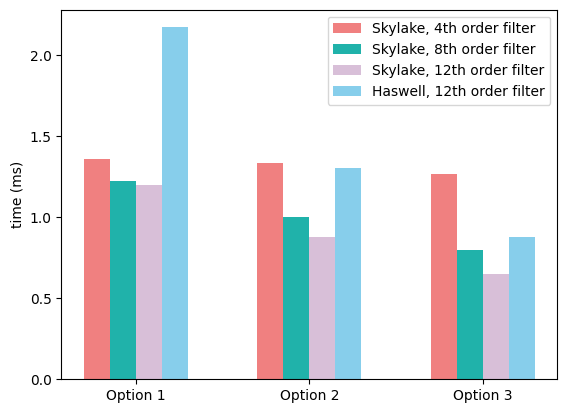
\includegraphics[width=3.3in]{real_time_test.png}}
    \caption{The real time for single second order option of filtering 1M samples under different order of filters and micro-architectures}
    \label{fig:Real_time_test}
  \end{figure}

Figure \ref{fig:Real_time_test} illustrates the real time for one second order option
of filtering 1.024M samples under different order of filters and micro-architectures. For example,
the red bar under option 1 shows the average time for each option 1 of filtering 1.024M samples under 
the fourth order system cascaded by 2 option 1 and with the Skylake CPU. 
By comparing with any three bars of options in the same color, we see the time spent for options has a decreasing order
by option 1, option 2 and 3, which fits the result of CPS in Table \ref{table:number_of_instructions_in_clock_cycles}. 
Together with Table \ref{table:number_of_instructions_in_clock_cycles}, 
we can also see the efficiency of our algorthm is improved by newer version of CPU.
Furthermore, an important observation is that if we compare the gaps between time spent for different order of systems under option 1
and those under option 3, we also verify the previous conclusion that our proposed algorithm will be more efficient for building a higher order filter.
By zooming in the bar with the shortest time in Figure \ref{fig:Real_time_test},
it shows under a Skylake CPU based system, the throughput of a 12th order recursive filter built by
cascading all second order options of our proposed algorithm can go up to above 260 MS$\slash$s, which is very efficient.













% To measure the performance of our proposed algorithm, we consider a general PC by using only single CPU and thread.
% The SIMD operation is realized via C++ programming and by the mean of vector class library (VCL).
% In VCL, two lengths of SIMD vectors can be used, i.e., 4 and 8. To get the better parallelism,
% we choose $M=8$. Recall that the matrix of data passed through the proposed functions is of size $M$ by $M$.

% \subsection{Rounding Error Issue}

% should we put the discussion of rounding error issue here or before the proposed algorithm?
% may be latter. Thus now I just show the particular solution.

